\documentclass[thesis,tocnosub,noragright,centerchapter,12pt]{uiucecethesis09}

% Use draftthesis for notes and date markings on every page.  Useful when you
%   have multiple copies floating around.
% Use offcenter for the extra .5 inch on the left side. Needed with fullpage and fancy.
% Use mixcasechap for compatibility with hyperref package, which does NOT like all caps default
% Use edeposit for the adviser/committee on the title page.
% Use tocnosub to suppress subsection and lower entries in the TOC.
% PhD candidates use "proquest" for the proquest abstract.

\makeatletter

%%%%%%%%%%%%%%%
% MK Added to make bib work
% MK removed on 1/8/19
% \bstctlcite{IEEEexample:BSTcontrol}

% MK added to highlight stuff
\usepackage{color,soul}

% MK added so figures can use the [H] option and be put where I want them.
\usepackage{float}

% MK added so algorithms work
\usepackage{algorithm}

%%%%%%%%%%%%%%%

\setcounter{secnumdepth}{5} % to make subsubsections work
\usepackage{setspace}
\usepackage{epsfig}  % for figures
\usepackage{graphicx}  % another package that works for figures
\usepackage{subfigure}  % for subfigures
\usepackage{amsmath}  % for math spacing
\usepackage{amssymb}  % for math spacing
%\usepackage{url}  % Hyphenation of URLs.
\usepackage{lscape}  % Useful for wide tables or figures.
\usepackage[justification=raggedright]{caption}	% makes captions ragged right - thanks to Bryce Lobdell


\DeclareMathOperator*{\argminA}{arg\,min} % Jan Hlavacek

% Uncomment the appropriate one of the following four lines:
%\msthesis
\phdthesis
%\otherdoctorate[abbrev]{Title of Degree}
%\othermasters[abbrev]{Title of Degree}

\title{Automated Isotope Identification Algorithm Using Artificial Neural Networks}
\author{Mark Kamuda}
\department{Nuclear Plasma and Radiological Engineering}
%\department{\mbox{Nuclear, Plasma, and Radiological Engineering}}
\degreeyear{2019}

% Advisor name is required for
% - doctoral students for the ProQuest abstract
% - master's students who do not have a master's committee
% \advisor{Assistant Professor Clair J. Sullivan}

% Uncomment the \committee command for
% - all doctoral students
% - master's students who have a master's committee
\committee{Kathryn Huff, Adviser\\
        Rizwan Uddin\\
        Tomasz Kozlowski\\
        Clair Sullivan\\
        Mark Hasagawa-Johnson}





\begin{document}

%%%%%%%%%%%%%%%%%%%%%%%%%%%%%%%%%%%%%%%%%%%%%%%%%%%%%%%%%%%%%%%%%%%%%%%%%%%%%%%
% COPYRIGHT
%
%\copyrightpage
%\blankpage

%%%%%%%%%%%%%%%%%%%%%%%%%%%%%%%%%%%%%%%%%%%%%%%
%%%%%%%%%%%%%%%%%%%% TITLE %%%%%%%%%%%%%%%%%%%%
%%%%%%%%%%%%%%%%%%%%%%%%%%%%%%%%%%%%%%%%%%%%%%%
\maketitle
%\raggedright
\parindent 1em%
\frontmatter

%%%%%%%%%%%%%%%%%%%%%%%%%%%%%%%%%%%%%%%%%%%%%%%
%%%%%%%%%%%%%%%%%%% ABSTRACT %%%%%%%%%%%%%%%%%%
%%%%%%%%%%%%%%%%%%%%%%%%%%%%%%%%%%%%%%%%%%%%%%%
\begin{abstract}
There is a need to develop an algorithm that can identify and quantify isotopes in low-resolution gamma-ray spectra. Trained gamma-ray spectroscopists typically rely on intuition when identifying isotopes in spectra. Because they incorporate something similar to the intuition used by trained spectroscopists, pattern recognition algorithms such as neural networks are prime candidates for automated isotope identification. Algorithms based on feature extraction such as peak finding or ROI algorithms work well for well-calibrated high resolution detectors. For low-resolution detectors, it may be more beneficial to use algorithms that incorporate more abstract features of the spectrum. To investigate this, an artificial neural network (ANN) was trained to predict the presence and relative activities of isotopes from gamma-ray spectra. The ANN is trained with simulated gamma-ray spectra, allowing easy expansion of the library of target isotopes. This proposal outlines extensions to this work including investigating new datasets and ANN structures.
\end{abstract}


%%%%%%%%%%%%%%%%%%%%%%%%%%%%%%%%%%%%%%%%%%%%%%%
%%%%%%%%%%%%%%%%%% DEDICATION %%%%%%%%%%%%%%%%%
%%%%%%%%%%%%%%%%%%%%%%%%%%%%%%%%%%%%%%%%%%%%%%%
%\begin{dedication}
%To my parents, for their love and support.
%\end{dedication}

%%%%%%%%%%%%%%%%%%%%%%%%%%%%%%%%%%%%%%%%%%%%%%%
%%%%%%%%%%%%%%% ACKNOWLEDGMENTS %%%%%%%%%%%%%%%
%%%%%%%%%%%%%%%%%%%%%%%%%%%%%%%%%%%%%%%%%%%%%%%
\begin{acknowledgments}
Acknowledgments text. 
\end{acknowledgments}

%%%%%%%%%%%%%%%%%%%%%%%%%%%%%%%%%%%%%%%%%%%%%%%
%%%%%%%%%%%%%% TABLE OF CONTENTS %%%%%%%%%%%%%%
%%%%%%%%%%%%%%%%%%%%%%%%%%%%%%%%%%%%%%%%%%%%%%%
\tableofcontents

%%%%%%%%%%%%%%%%%%%%%%%%%%%%%%%%%%%%%%%%%%%%%%%
%%%%%%%%%%%%%%% LIST OF TABLES %%%%%%%%%%%%%%%%
%%%%%%%%%%%%%%%%%%%%%%%%%%%%%%%%%%%%%%%%%%%%%%%
% The List of Tables is not strictly necessary. Omitting the List of Tables will
% simplify the thesis check and reduce the number of corrections.
\listoftables

%%%%%%%%%%%%%%%%%%%%%%%%%%%%%%%%%%%%%%%%%%%%%%%
%%%%%%%%%%%%%%% LIST OF FIGURES %%%%%%%%%%%%%%%
%%%%%%%%%%%%%%%%%%%%%%%%%%%%%%%%%%%%%%%%%%%%%%%
% The List of Figures is not strictly necessary. Omitting the List of Figures will
% simplify the thesis check and reduce the number of corrections.
\listoffigures

%%%%%%%%%%%%%%%%%%%%%%%%%%%%%%%%%%%%%%%%%%%%%%%
%%%%%%%%%%% LIST OF ABBREVIATIONS %%%%%%%%%%%%%
%%%%%%%%%%%%%%%%%%%%%%%%%%%%%%%%%%%%%%%%%%%%%%%
% The List of Abbreviations is not strictly necessary.
%\chapter{LIST OF ABBREVIATIONS}

%\begin{symbollist*}
%\item[DNN] Dense Neural Network
%\item[CNN] Convolution Neural Network
%\end{symbollist*}

%%%%%%%%%%%%%%%%%%%%%%%%%%%%%%%%%%%%%%%%%%%%%%%
%%%%%%%%%%%%%% LIST OF SYMBOLS %%%%%%%%%%%%%%%%
%%%%%%%%%%%%%%%%%%%%%%%%%%%%%%%%%%%%%%%%%%%%%%%
%\begin{symbollist}[0.7in]
%\item[$\tau$] Time taken to drink one cup of coffee.
%\end{symbollist}

\mainmatter

%%%%%%%%%%%%%%%%%%%%%%%%%%%%%%%%%%%%%%%%%%%%%%%
%%%%%%%%%%%%%%%%%%%%%%%%%%%%%%%%%%%%%%%%%%%%%%%
%%%%%%%%%%%%%%%%%%%%%%%%%%%%%%%%%%%%%%%%%%%%%%%
%%%%%%%%%%%%%%%% THESIS BODY %%%%%%%%%%%%%%%%%%
%%%%%%%%%%%%%%%%%%%%%%%%%%%%%%%%%%%%%%%%%%%%%%%
%%%%%%%%%%%%%%%%%%%%%%%%%%%%%%%%%%%%%%%%%%%%%%%
%%%%%%%%%%%%%%%%%%%%%%%%%%%%%%%%%%%%%%%%%%%%%%%

\chapter{Introduction}

\section{Introduction and Motivation}

Gamma-ray spectroscopy is an important part of homeland security and nonproliferation technologies. By analyzing the gamma-ray spectrum of some material, a user can determine the isotopes present and their relative quantities. This technique can be used to differentiate special nuclear materials (SNM) such as weapons grade plutonium from a benign medical or industrial source in a cargo container. Gamma-ray spectroscopy can also be used to measure the enrichment of uranium, an important measurement for nonproliferation and nuclear treaty verification. 

Typically, gamma-ray spectroscopy is performed by a trained operator \cite{burr2009} or a hand-held radioisotope identification device (RIID). Because RIID users are usually not trained to analyze gamma-ray spectra, the U.S. DOE (Department of Energy) employs a team of on-call spectroscopists to resolve alarms created by RIIDs. Despite their importance, reported performance of commercial RIIDs are generally poor \cite{pibida2004,blackadar2003,blackadar2004}. It has been argued that RIID improvements fall into two categories \cite{swoboda2004}: improvements in the detection materials and improvements in the identification algorithms \cite{blackadar2003}. Detection materials can be improved by reducing the cost of producing large detector volumes for advanced detection materials \cite{Gostilo2004,Chen2018} or by finding new room-temperature gamma-ray detection materials with high intrinsic efficiency and resolution comparable to high purity germanium (HPGe) semiconductor detectors \cite{swoboda2004}. While these advanced materials can be used to improve performance, commercial RIIDs typically employ the medium-resolution material sodium iodide (NaI) or high-resolution materials like HPGe and cadmium zinc tellurium (CZT). High-resolution materials do offer better performance, but these materials suffer from several drawbacks. Drawbacks like material cost, requirement for cryogenic temperatures (for HPGe), and difficulty creating large detector volumes. Despite the drop in resolution, the medium-resolution detection material NaI is still standard in the RIID industry due to its ease of use, low cost, large detector volumes, high intrinsic efficiency, high light output, and acceptable resolution for gamma-ray spectroscopy \cite{swoboda2004}. It has been argued that the focus of improving RIIDs should focus on the identification algorithms using this industry standard material \cite{blackadar2003}. Because of the reasons outlined above, the focus of this dissertation is to investigate a novel detection method, machine learning algorithms, as a possible avenue of improving the performance of RIIDs using NaI.

The medium-resolution detector of interest in this work is the Ortec 905-3 2- x 2-in. NaI cylindrical scintillation detector \cite{Hofstadter1948}. Despite it's widespread use, NaI detectors have several issues that complicate automated identification. The first issue is poor resolution compared to other more expensive radiation detection material, such as HPGe and CZT. The lower-resolution makes some photopeaks unresolvable from each other, complicating identification. The second issue is calibration drift due to voltage drift in detectors electronics and temperature changes \cite{knoll,gilmore}. This calibration drift changes the locations and shapes of features in a gamma-ray spectrum. Automatic recalibration can be accomplished through automatically calibrating to a built-in reference source or to a naturally occurring background source. These methods fall short for different reasons. Built-in sources need to be periodically replaced and add an unwanted signal to a spectrum. Calibrating off of a background reference, typically the 1460 keV gamma-ray peak from $^{40}$K, requires the signal-to-noise ratio of that photopeak to be significant. For short integration times common in homeland security measurements this is often be infeasible. 

The third issue is a non-linear energy response. This manifests as a small second order term in their calibration. This complicates. While not specific to NaI detectors, the fourth issue affecting identification algorithms is background radiation from naturally occurring radioactive material (NORM). Background radiation can change both in intensity and composition based on location and weather. This background signal can obscure features in gamma-ray spectra. Despite these drawbacks, our previous works have demonstrated ANNs capable of identifying multiple isotopes in unknown backgrounds with a wide range of calibration settings \cite{kamudaThesis2017,kamuda2017}.


% \section{Radioisotope Identification Device Applications}

% Statistical methods applied to gamma-ray spectroscopy algorithms in nuclear security missions \cite{Min2014}.

% \subsection{Homeland Security}

% Handheld RIIDs are used by boarder protection and law enforcement for porthole and area monitoring \cite{Hodge2007}. An example of area monitoring could be monitoring a high traffic area during a high-profile event. An example of porthole monitoring is monitoring cargo vehicles. RIIDs are typically employed in second screening activities, after a primary count rate alarm is triggered. In order to minimize traffic and ensure cargo containers leave in an economically reasonable time, screening activities are kept on the order of minutes. Another example of porthole monitoring is temporary checkpoints where traffic is slowed but not stopped. Often, the important task for devices employed in vehicle screening is determining if a primary alarm came from NORM, a legitimate industrial source, or SNM.


% \cite{fagan2012}

% GRADER PROGRAM https://www.dhs.gov/guidance-grader-program


% RIIDs also can be used to identify orphaned sources.
% https://www-sciencedirect-com.proxy2.library.illinois.edu/science/article/pii/S0969804302002221

% Pozzi great references https://www-sciencedirect-com.proxy2.library.illinois.edu/science/article/pii/S0168900217300074


% DATASET https://www-sciencedirect-com.proxy2.library.illinois.edu/science/article/pii/S0168900214012741

% \subsection{Nuclear Treaty Verification}

% Talk about Zero knowledge measurements 


\section{Neural Network History}


Artificial neural networks were first theorized in the 1940s as a model of how complex biological systems like groups of neurons learn and remember \cite{Pitts1943, Hebb1949}. These theories hypothesized that learning took place by reinforcing neural connections corresponding to some correct behavior that was reinforced. The first implementation of an ANN came in 1958 in the form of The Perceptron \cite{Rosenblatt1958, Rosenblatt1962}. The Perceptron was a single layer neural network implemented in a two-class image recognition problem. A class is a unique category, like dog and cat or on and off. There is no limit on the number of classes a model can attempt to learn. Another single layer neural network design was ADALINE, created in 1960 \cite{Widrow1960}. While the ADALINE algorithm shares a similar architecture with the perceptron, the learning rule is different. Unfortunately, the single-layer perceptron was proven to not work in cases where classes in the data are not linearly separable \cite{Minsky1969}. This realization led to a decline in neural network research.

While a single layer network could only solve linearly separable problems, in 1969 it was also found that a network with multiple layers could solve problems that are non-linearly separable \cite{Minsky1969}. The perceptron algorithm was limited to a single layer network due to its activation function being a non-differentiable step function. It was soon shown that multiple ADALINE neurons could be stacked on top of each other, creating a MADALINE network \cite{Ridgway1962}. Due to its multilayer structure, MADALINE is able to learn non-linearly separable functions. A MADALINE network was used as an adaptive filter that removes echo from phone lines \cite{Widrow1988}.

Further advances in ANNs came in the form of learning improvements. Not long after the success of ADALINE and MADALINE, it was suggested that the concept of error propagation could be applied to ANNs \cite{Werbos1974, Rumelhart1986}. Additionally, it was shown that error backpropogation applied with a differentiable non-linear activation function was an extremely powerful method to train ANNs \cite{Murtagh1991}. Algorithms based on the backpropogation of error are now the most common method to train ANNs.

Currently, ANNs can solve many diverse problems. ANNs have shown promise in everyday problems such as handwritten zip code recognition \cite{LeCun1989}, image recognition \cite{Krizhevsky2012}, and fingerprint identification \cite{Jeyanthia2015}; as well as more complicated problems such as lung cancer classification based on MRI images \cite{Selvakumari2016}, estimating surface soil moisture from high-resolution aerial images of cropland \cite{Hassan-Esfahani2015}, and stock market forecasting \cite{Rababaah2015}.


\section{Gamma-Ray Spectroscopy for Isotope Identification}

Traditionally, isotope identification is conducted by a trained spectroscopist. Rawool-Sullivan et al. identified a common workflow performed by a group of gamma-ray spectroscopists \cite{Sullivan2010}. This workflow includes discriminating background and source photopeaks, adjusting the calibration using background photopeaks and checking for shielding effects in the low-energy photopeaks. Once photopeaks are identified, the spectroscopist would use their prior knowledge of isotope emissions (or consult a database of these emissions) to match isotopes to the spectrum. The researchers also noted that while  spectroscopists used this book knowledge, they often would use intuition developed from analyzing tens or hundreds of gamma-ray spectrum. The researchers also noted the difficulty in incorporating this subjective analysis into an automated algorithm.
% This is one of the main arguments for using ANNs in automated isotope ID


There are many automated radioisotope identification methods available, but few perform well given a low-resolution gamma-ray spectrum of a mixture of radioisotopes. Common methods include library comparison algorithms, region of interest (ROI) algorithms, principle component analysis (PCA), and template matching.

Library comparison algorithms attempt to match photopeak energies found in a gamma-ray spectrum with those found in a library of known isotope decay energies. Drifts and uncertainties in detector calibration can lead to misidentifying photopeaks, leading to incorrect isotope identifications \cite{burr2009}. To be automated, this method needs an algorithm to extract photopeak centroids despite calibration drift and an unknown background signal. While methods for photopeak extraction exist and are actively researched \cite{mariscotti1967,DELOTTO1977,GARDNER2011}, they face difficulties when a large number of photopeaks overlap in a spectrum \cite{xiong2015}, such as when a mixture of radio-isotopes are measured with a low-resolution detector .

ROI algorithms define regions in a spectrum where target radioisotope photopeaks are expected. Counts in these regions are then compared to a measured or expected background. Significant elevation in counts in a target isotopes ROI's indicates the presence of that isotope. ROI algorithms operate poorly when photopeaks of different radioisotopes overlap \cite{burr2009}. Because of this, large isotope libraries perform poorly using this method. Similarly to the library comparison algorithm, calibration drift may shift photopeaks into neighboring ROIs, leading to incorrect identification. The ROI method has been used to differentiate normally occurring radioactive material (NORM) from special nuclear material (SNM) using plastic scintillators \cite{Ely2006}.

PCA can also be applied to radioisotope identification. The goal of PCA is to reduce the dimensionality of a dataset into uncorrelated variables \cite{Jolliffe2002}. Using a few of these principle components, the data may be represented in a reduced space that contains most of the information present in the original data. The transformed data can then be clustered based on isotope identity. Clustering algorithms may include K-means or Mahalanobis distance \cite{Kanungo2002, Kumari2012}. PCA has been applied to isotope identification using plastic scintillators \cite{Boardman2012} and anomaly detection using both plastic scintillators and NaI detectors \cite{runkle2006b}. Despite the progress of PCA in some isotope identification problems, there has not been significant progress in applying PCA to separating mixtures of isotopes in gamma-ray spectra.

Template matching algorithms find an example in a database of gamma-ray spectra that most closely matches a measured spectrum \cite{burr2009}. The database of spectra can contain multiple detector calibration settings, shielding materials, and source-to-detector distances. Goodness of fit can be measured using a hypothesis test such as chi-squared test, euclidean distance, or Mahalanobis distance. While a sufficient amount of example spectra can be used to identify almost any measured spectrum, the drawback of this method is the time necessary to compare a measured spectrum to the library and the computer memory necessary to store said library. This method also may have difficulty when mixtures of isotopes are considered, although work is being done to correct this \cite{mattingly2010}.

These algorithms largely incorporate book knowledge. By further incorporating the intuition identified by Rawool-Sullivan et al., these algorithms may be improved. By carefully creating a training set of spectra and intelligently applying deep learning architectures, a machine learning approach to automated gamma-ray spectroscopy may be able to marry book knowledge and a trained spectroscopists intuition.


\section{Automated Isotope Identification Using ANNs}

There have been a number of published papers which apply ANNs to automated isotope identification. ANNs have been applied to peak fitting \cite{Abdel-Aal2002}, isotope identification \cite{Abdel-Aal1996, Medhat2012}, and activity estimation \cite{Abdel-Aal1996, Vigneron1996}. 

Peak fitting methods include applying 


Many of these works rely on ROI methods \cite{Pilato1999}, feature extraction \cite{Chen2009}, high-resolution gamma-ray spectra as the input to the ANN \cite{Yoshida2002}, small libraries of isotopes, and assume perfectly calibrated detectors. ANN training methods created for high-resolution gamma-ray spectra may not perform well when trained using low-resolution spectra. Because of the large discrepancy in resolution, the features exploited by a ANN trained on high-resolution spectra would be different than low-resolution spectra. In addition to this, ANN training that relies on ROI methods may not perform well when ROIs overlap significantly with large libraries of isotopes. Feature extraction and ROI methods may also falter when the background radiation field is unknown or the detector's calibration is unreliable.  

% ANNs using feature extraction on 3x3 NaI detector \cite{HE2018}.

\section{Chapter Conclusion}

There are two main questions addressed in this work. The first is question addresses what physics should be incorporated into a synthetic dataset of gamma-ray spectra for different problems in isotope identification and quantification. The second question addresses how different ANNs architectures perform on these datasets. Gamma-ray spectroscopists often use intuition when identifying isotopes in spectra. ANNs mimic this abstract analysis, synthesizing features of a gamma-ray spectrum in non-intuitive ways. Exploiting this intuition may overcome common hurdles encountered by other isotope identification algorithms.

To overcome the issues outlined above, instead of training an ANN using predetermined ROIs or feature extraction, it may be better to train the ANN with an entire gamma-ray spectrum. Due to perceived training issues and computational requirements associated with using the entire spectrum \cite{Pilato1999,Yoshida2002}, this approach has been avoided in previous works. Despite this, it has been shown that training an ANN using the full spectrum is a viable method to identify and quantify isotopes in gamma-ray spectra \cite{kamuda2017,kamudaThesis2017,kamuda2018}. There is also evidence that this method can overcome common  gamma-ray spectroscopy issues like gain shifts due to changes in temperature and identifying isotopes in spectra without clear isotopic features.

The solution outlined in this work is to perform radioisotope identification and quantification simultaneously using an ANN. Skipping automated peak-fitting routines releases the algorithm from the burden of determining proper peak-fitting subroutines for the variety of cases in which a peak may be seen. A photopeak can typically be fit using a Gaussian distribution added to a linear baseline. This baseline changes based on its location in another photopeak's Compton continuum. In spectra where peaks overlap, deconvolution techniques may be needed to resolve constituent peaks. An unknown gain or poorly calibrated detector will shift photopeaks, further complicating a spectrum. Instead of making deterministic rules for each of these cases, a machine learning algorithm can be taught to recognize and handle them automatically.

Traditionally, once photopeaks are found, another algorithm is needed to measure the locations of peak centroids and additional information (peak area, area uncertainty) to identify what isotopes are present in a spectrum. This process adds computation time and again suffers from the need to be modified to handle changes in a spectrum as described above. Also, the algorithm that performs identification based on peak information must be tailored to the peak-fitting routine. This requires unique algorithms to be created for different detector materials and sizes, as they change the shape of the spectrum. Using an ANN with an appropriate training set, these problems can be avoided.

By allowing a machine to learn the important features of a gamma-ray spectrum, the problem of determining the best analysis technique given a spectrum with significant features overlap and unknown calibration is avoided. This method is ideal for low-resolution gamma-ray spectroscopy for mixtures of radioisotopes for a number of reasons. Because this method uses simulated gamma-ray spectra to train the ANN, there is no restriction on the number of isotopes allowed in the library or their identity. This allows the ANN training set to be cheaply generated using mixtures of exotic, dangerous, or short-lived isotopes that are not easily accessible in an academic setting. 

Another benefit of using a training set of simulated spectra is that an ANN may be trained for a specific scenario using a custom isotope library. The isotope library requirements for a border patrol, which may focus on distinguishing possibly shielded medical isotopes and NORM from SNM, are very different from the isotope library needed to perform post-detonation nuclear forensics. Because spectra can be generated with different calibrations, this method can be insensitive to a range of calibration shifts due to temperature change or operator error. This insensitivity would allow isotope identification and quantification to be performed without prior knowledge of the detectors calibration.

Experiments in this work fall into two categories: advanced simulated datasets and advanced machine learning architectures. The first advanced dataset is based on the the American National Standards Institute performance criteria for hand-held instruments for the detection and identification of radionuclides, ANSI N42-34-2006 \cite{ANSI}. This dataset will incorporate the effects of shielding, calibration drift, and unknown background. The second dataset will be based on a zero knowledge measurement for automated uranium enrichment calculations. The performance of models trained on both datasets will be assessed on a series of real and simulated gamma-ray spectra. The machine learning architectures explored will include a dense neural network (DNN), dense autoencoder (DAE), convolutional neural networks (CNNs), and convolutional autoencoder (CAE).


\chapter{Theory}

\section{Gamma-ray Spectroscopy}



\subsection{Detector Efficiency}

The following sections describe intrinsic mechanisms that remove counts from the full-energy peak. Absolute efficiency is also affected by shielding material and source-to-detector distance.

\subsubsection{Compton Scattering}

\subsubsection{Photoelectric effect}

\subsubsection{Pair Production}



\subsection{Energy Resolution}


\begin{figure}[H]
\centering
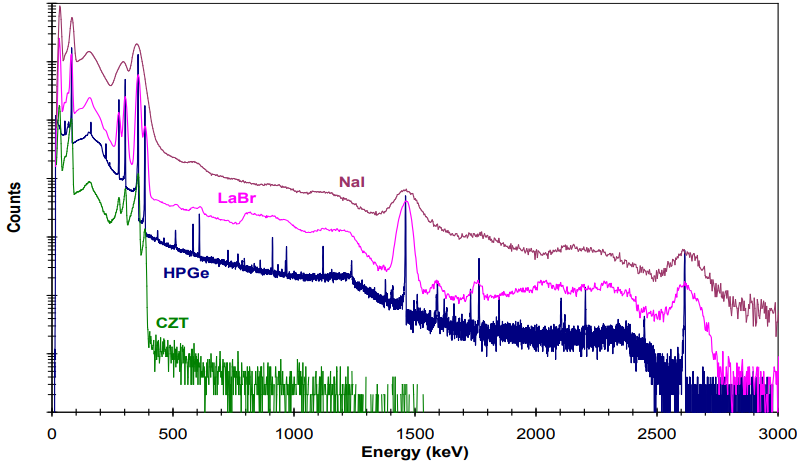
\includegraphics[width=0.95\linewidth]{images/Ba133_spectrum_different_detector_materials_Market_Survey_Report}
\caption{Ba133 spectrum measured using different detector materials \cite{RIIDMarketSurveyReport}.}
\label{fig:uranium_concentration}
\end{figure}


\subsection{Background Effects}


% Air Survey on Background Gradients https://www-sciencedirect-com.proxy2.library.illinois.edu/science/article/pii/S0265931X13002373

\begin{figure}[H]
\centering
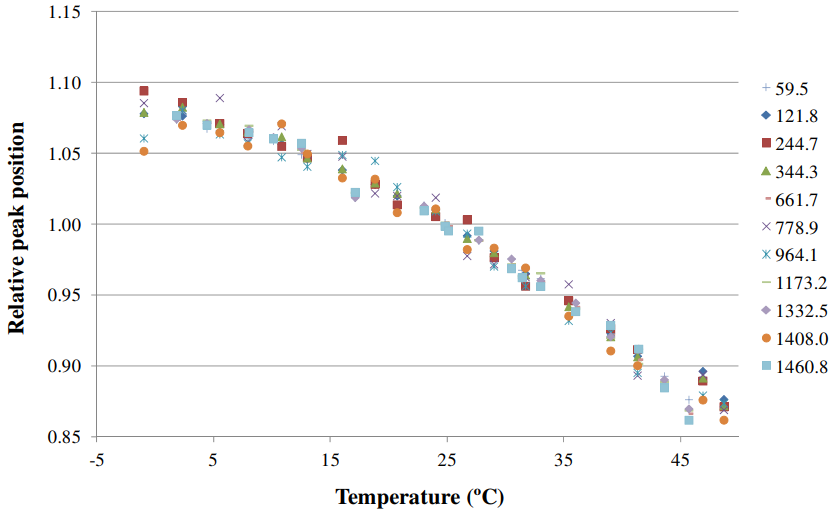
\includegraphics[width=0.95\linewidth]{images/temp_vs_relative_peak_position_CASANOVAS2012588}
\caption{Map of uranium concentrations in the United States.}
\label{fig:uranium_concentration}
\end{figure}


% \USGS Open-File Report 2005-1413: Terrestrial Radioactivity and
%Gamma-ray Exposure in the United States and Canada," 2013.
% [Online]. Available: http://pubs.usgs.gov/of/2005/1413/maps.htm


\subsection{Affect of Temperature Change on Calibration}


Figure \ref{fig:CASANOVAS2012588} shows how relative peak position shifts with respect to changes in temperature of an ORTEC Model 905-3 2x2 NaI detector. Gain stabilization methods rely on 

\begin{figure}[H]
\centering
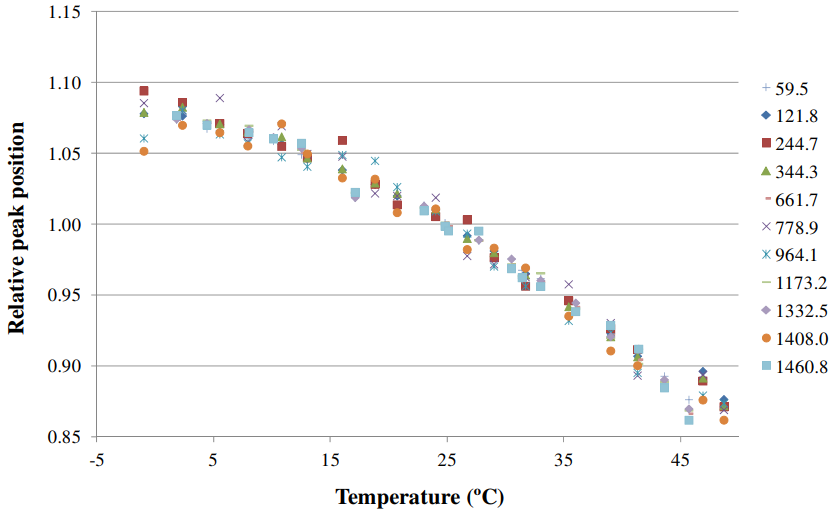
\includegraphics[width=0.95\linewidth]{images/temp_vs_relative_peak_position_CASANOVAS2012588}
\caption{Temperature vs relative photopeak position for an ORTEC Model 905-3 2x2 NaI detector \cite{CASANOVAS2012588}.}
\label{fig:CASANOVAS2012588}
\end{figure}




\section{Machine Learning}

In this section, neural network architectures and parameters that effect training will be described. Neural network architectures will include DNN, CNN, and the autoencoder. 

\subsection{Neural Network Architecture}

% Node/neruon, get this lingo straight here
An ANN is a mathematical model that attempts to map an arbitrary function from $\mathbb{R}^M$ to $\mathbb{R}^N$, where $M$ and $N$ are positive integers. An ANN accomplishes this by mimicking biological neurons. One example of an ANN architecture is shown in Figure \ref{fig:Network}. This ANN has N neurons in input layer A, J neurons in hidden layer B, and K neurons in output layer C. Each neuron in adjacent layers are connected by weights, represented in Figure \ref{fig:Network} by arrows connecting neurons. 


\begin{figure}[H]
\centering
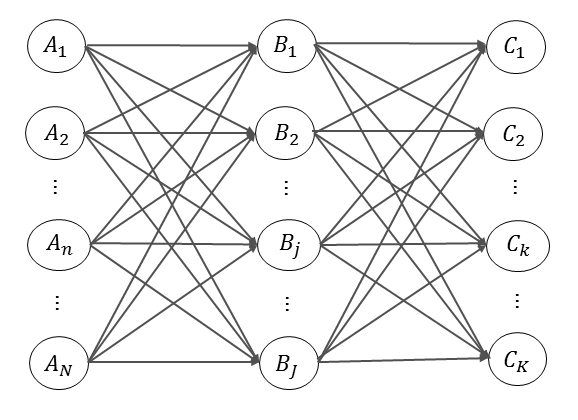
\includegraphics[width=0.75\linewidth]{images/Network}
\caption{Example ANN with input neurons $A_n$, hidden neurons $B_j$, and output neurons $C_k$.}
\label{fig:Network}
\end{figure}


Similar to a biological neuron, the ANN neuron receives input stimuli, performs an operation using it, and outputs the resulting signal. The structure and equation governing the operation of an individual neuron is shown in Figure \ref{fig:Node}. 

\begin{figure}[H]
	\centering
	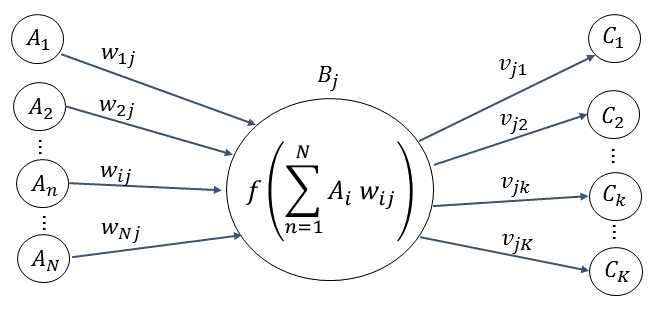
\includegraphics[width=0.75\linewidth]{images/Node_ABC_2}
	\caption{Summary of the operation of a single neuron.}
	\label{fig:Node}
\end{figure}

As seen in Figure \ref{fig:Node}, each neuron operates by summing the products of the previous layers values ($A_1$, $A_2$, ... $A_N$}) and each individual weight ($w_{1j}$, $w_{2j}$, ... $w_{nj}$) connecting the neurons. This summation is analogous to the stimulus a biologic neuron receives from its dendrites. The stimulus is then operated on by an activation function $f$, typically a non-linear function. The output signal is then passed to the next layer of the ANN where the process repeats. An ANN may be trained by setting the network weights, $\mathbf{W}$, in such a way that they minimize the error between target values, $\mathbf{T}$, in a training dataset, $\mathbf{Y}$, and the ANN output given that training dataset, $f( \mathbf{Y} ; \mathbf{W} )$, 
%
\begin{equation} \label{eq:argminW_Error}
\underset{\mathbf{W}}{\text{argmin}} {\text{ Error}}(f(\mathbf{Y} ; \mathbf{W} ) , \mathbf{T} ).
\end{equation}
% \underset{w}{\text{argmin}} \sum_{i=1}^{N} \Vert t_i - y_i \Vert^2
Except under simple cases, Equation \ref{eq:argminW_Error} cannot be solved analytically. Numerical methods for solving this equation include gradient descent through the back-propagation of errors \cite{Rumelhart1986}, genetic learning algorithms \cite{Yao1999}, and Newtons method \cite{Fletcher2000}.


\subsection{Simple Neural Network Example}

An example of a very simple one-layer ANN is shown in Figure \ref{fig:one_layer_net}. This ANN takes two inputs ($x_1$ and $x_2$) and performs the operation shown in Figure \ref{fig:Node}. The weights in the hidden layer connecting the $i^{th}$ input neuron to the $j^{th}$ output neuron will be represented by $w_{ij}$. The bias is set to a constant value of 1. This allows the bias to be effectively trained by changing the weights connecting the bias to the next layer. Using the hyperbolic tangent function, the network outputs for each class $y_1$, $y_2$, and $y_3$ range from -1 to 1. Using these outputs, any input can be classified into a given class if the class' respective output neurons value is above zero, or not in a class if the output neurons value is below zero. The equation for the output of the $j^{th}$ output is given in Equation \ref{eq:single_layer_eq_sum}, where $x_i$ is the $i^{th}$ input from the previous layer, and $b_i$ is the value of the weight connecting the $j^{th}$ output to the bias neuron.
%
\begin{equation} \label{eq:single_layer_eq_sum}
y_j = \tanh(\sum_i x_i w_{ij} + b_j),
\end{equation}

To more clearly understand the geometry of the network's operation, consider the dataset in Figure \ref{fig:training_set_one_layer}. This dataset is composed of three classes: red, green, and blue. The axes that define this dataset are the inputs to the single layer network in Figure \ref{fig:one_layer_net}, ($x_1$,$x_2$). If $\mathbf{W}$ is defined to be a vector with elements ($w_{11}$, $w_{21}$), a line can be defined perpendicular to $\mathbf{W}$ and shifted by $\frac{b_1}{||\mathbf{W}||}$ away from the origin in the direction of $\mathbf{W}$. Given appropriate values for $w_{11}$, $w_{21}$, and $b_1$, a line that separates the blue class from the non-blue class can be created. Any point on the -$\mathbf{W}$ side of the line will have $y_1 < 0$, allowing for classification. Similarly, a separating line for the red class using $w_{12}$, $w_{22}$, and $b_2$ and a separating line for the green class using $w_{13}$, $w_{23}$, and $b_3$ can be constructed. 

The classes in this example dataset are linearly separable, meaning lines can be drawn completely separating each class. If the classes were not linearly separable, additional hidden layers would be necessary to compute the function. It has been shown that additional hidden layers allow the creation of arbitrary decision boundaries \cite{Hornik1991}. 
%
\begin{figure}[H]
	\centering
	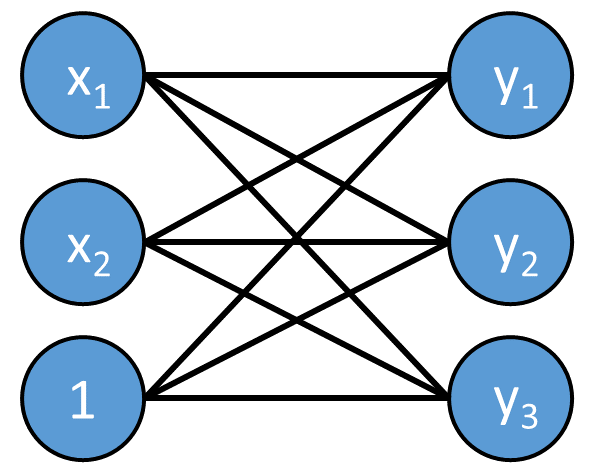
\includegraphics[width=0.45\linewidth]{images/One_layer_net_v31}
	\caption{Example of a single-layer neural network with two inputs ($x_{1}$ and $x_{2}$), three classes ($y_{1}$, $y_{2}$, $y_{3}$), and a bias neuron set to one.}
	\label{fig:one_layer_net}
\end{figure}
% Change these to diff objects to get around grey-scale thesis...?
%The neural network described in Figure \ref{fig:one_layer_net} has two inputs, so its decision boundaries are lines. If the network had three inputs each decision boundary is a plane. Given $N$ inputs, each decision boundary is a $N$-dimensional hyperplane. 


% \cite{Hornik1991} is universal approx theory for ANNs

% pics side by side better? Before and after hyperplane addition?

\begin{figure}[H]
	\centering
	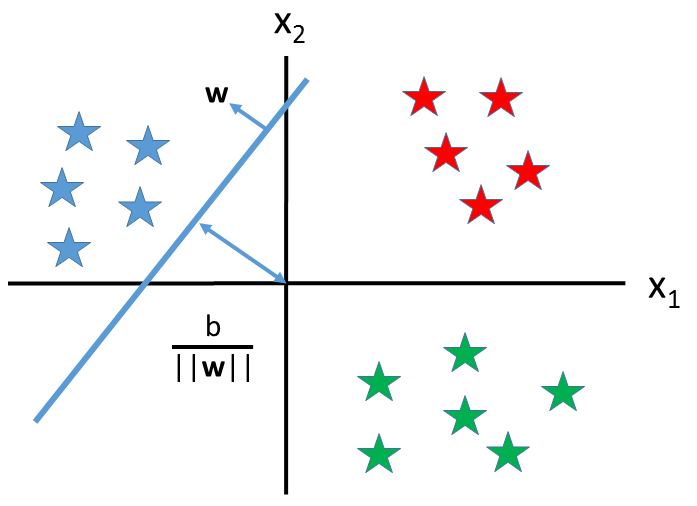
\includegraphics[width=0.65\linewidth]{images/training_set_for_single_layer_hyperplane_v2}
	\caption{One possible dataset describing a three class function. Each class is represented by a different color.}
	\label{fig:training_set_one_layer}
\end{figure}

\subsection{Neural Network Training}

One of the most common methods of training an ANN is through error backpropagation. Error backpropagation is a method to minimizes an error function with respect to the weights connecting neurons as seen in Equation \ref{eq:dMSE}. % If the error function is convex with respect to the network weights, the error with respect to the weights in the network can be minimized using its derivative. THIS IS WRONG. ANN with no hidden layers will have a purely convex error fctn wrt weights, add layers and we get local minima/maxima

Training the simple, one-layer ANN requires finding an expression for \ref{eq:dMSE}. For the following section, let $y_i$ be defined as in Equation \ref{eq:single_layer_eq_sum}, $E_{MSE}$ be defined as the mean squared error function, and training data be defined as in Equation \ref{eq:train_data_D} where $\bold{x_n}$ represents the $n^{th}$ training token and $t_n$ represents the $n^{th}$ binary training target \cite{Nielsen2015}. Note, this derivation would need to be repeated for a different error function. By the chain rule,
%
\begin{equation} \label{eq:dMSE}
\frac{dE_{MSE}}{dw_j} = \frac{dE_{MSE}}{dy_i} \frac{dy_i}{dw_j}.
\end{equation}
%
\begin{equation} \label{eq:train_data_D}
 D={(\boldsymbol{x}_1,t_1), ... ,(\boldsymbol{x}_n,t_n)}
\end{equation}
Equation \ref{eq:dMSE} can be solved by first evaluating $\frac{dE_{MSE}}{dy_i}$,
%
\begin{equation} \label{dE_{MSE}/dy_i}
\frac{dE_{MSE}}{dy_i}  = \frac{d}{dy_i} \sum_i(t_i - y_i)^2
\end{equation}
%
\begin{equation} \label{dE_{MSE}/dy_i}
 = \sum_i  \frac{d}{dy_i} (t_i - y_i)^2
\end{equation}
%
\begin{equation} \label{eq:MSE_deriv}
 =  -2 \sum_i  (t_i - y_i).
\end{equation}
%
Evaluating $\frac{dy_i}{dw_j}$,
%
\begin{equation} \label{dE_{MSE}/dy_i}
\frac{dy_i}{dw_j}  = \frac{d}{dw_j} \tanh( \boldsymbol{w}' \boldsymbol{x}_i + b) 
\end{equation}
%
\begin{equation} \label{dE_{MSE}/dy_i}
 = \tanh'( \boldsymbol{w}' \boldsymbol{x}_i + b) \frac{d}{dw_j}( \boldsymbol{w}' \boldsymbol{x}_i + b)
\end{equation}
%
\begin{equation} \label{dE_{MSE}/dy_i}
 = \tanh'( \boldsymbol{w}' \boldsymbol{x}_i + b)  x_{ij}.
\end{equation}
%
\noindent where $x_{ij}$ is the $j^{th}$ feature of the $i^{th}$ training vector.
%
The update rule for the bias vector is found using
%
\begin{equation} \label{eq:ladidadi}
\frac{dE_{MSE}}{db_j} = \frac{dE_{MSE}}{dy_i} \frac{dy_i}{db_j}.
\end{equation}
%
The expression for $\frac{dE_{MSE}}{dy_i}$ is known from Equation \ref{eq:MSE_deriv}. Evaluating the other derivative in \ref{eq:ladidadi},
%
\begin{equation} \label{dE_{MSE}/dw_j}
\frac{dy_i}{db_j} = \frac{d}{db_j} \tanh(\boldsymbol{w}'\boldsymbol{x}_i + b),
\end{equation}
%
\begin{equation} \label{dE_{MSE}/dy_i}
 = \tanh'( \boldsymbol{w}' \boldsymbol{x}_i + b).
\end{equation}
%
Finally, the gradient of the error function with respect to a single weight can be computed, 
%
\begin{equation} \label{eq:dE_{MSE}/dw_j_final}
\frac{dE_{MSE}}{dw_j} =  -2 \sum_i  (t_i - y_i) \tanh'( \boldsymbol{w}' \boldsymbol{x}_i + b)  x_{ij},
\end{equation}
%
and a single bias,
%
\begin{equation} \label{eq:dE_{MSE}/db_j_final}
\frac{dE_{MSE}}{db_j} =  -2 \sum_i  (t_i - y_i) \tanh'( \boldsymbol{w}' \boldsymbol{x}_i + b).
\end{equation}
%
The derivative in Equations \ref{eq:dE_{MSE}/dw_j_final} and \ref{eq:dE_{MSE}/db_j_final} can used to update each weight and bias in the network as defined by 
%
\begin{equation} \label{eq:update1}
\Delta w_{j} = - \eta \frac{dE_{MSE}}{dw_j}
\end{equation}
%
and 
%
\begin{equation} \label{eq:update2}
\Delta b_{j} = - \eta \frac{dE_{MSE}}{db_j}
\end{equation}
%
where $\eta$ in Equations \ref{eq:update1} and \ref{eq:update2} represents the learning rate of the neural network. The learning rate and its effect on training will be discussed more thoroughly in a later section.

Gradient descent can also be applied to multi-layer ANN. Given an L-layer network where the input stimuli to the $l^{th}$ layer training example x is represented by
%
\begin{equation} \label{eq:CrossEntropy}
\boldsymbol{z}^{x,l} = \boldsymbol{w}^{l}  \boldsymbol{a}^{x,l-1} + \boldsymbol{b}^{l}
\end{equation}
%
where $\boldsymbol{w}^{l}$ is the $l^{th}$ layer's weight matrix, $\boldsymbol{b}^{l}$ is the $l^{th}$ layer's bias vector, and the output activation vector from the $(l-1)^{th}$ layer is 
%
\begin{equation} \label{eq:CrossEntropy}
\boldsymbol{a}^{x,l-1} = f^{l-1}(\boldsymbol{z}^{x,l-1})
\end{equation}
%
where $f^{l-1}$ represents the non-linear activation function used in the $(l-1)^{th}$-layer. Defining the output error as 
%
\begin{equation} \label{eq:CrossEntropy}
\delta^{x,L} = \frac{\partial C}{\partial a^{x,L}} \odot \frac{\partial f^{l-1}(\boldsymbol{z}^{x,l-1}) }{\partial \boldsymbol{z}^{x,l-1}}, 
\end{equation}
%
where $\odot$ is the Hadamard product, the output error can backpropagate to previous layers. For each $l=L-1,L-2,...,2$ an error can be defined by
%
\begin{equation} \label{eq:CrossEntropy}
\delta^{x,l} = ((\boldsymbol{w}^{l+1})^T \delta^{l+1}) \odot \frac{\partial f^{l}(\boldsymbol{z}^{x,l}) }{\partial \boldsymbol{z}^{x,l}}.
\end{equation}
%
The gradient of the cost function as a function of each individual weight and bias can now be defined as 
%
\begin{equation} \label{eq:CrossEntropy1}
\frac{\partial E}{\partial w_{jk}} = a^{l-1}_k \delta^l_j
\end{equation}
%
and 
%
\begin{equation} \label{eq:CrossEntropy2}
\frac{\partial E}{\partial b_j} = \delta^l_j.
\end{equation}
%
Using Equations \ref{eq:update1} and \ref{eq:update2}, the weights can be updated for a single iteration of backpropogation. 

ANNs require some stopping condition to conclude training. One simple stopping condition is ending training when a threshold in network accuracy on a testing set is reached. Where this simple accuracy test is not applicable, such as for regression training sets, a condition based on the ANN training error metric can be used.

Early stopping has the benefit of preventing overfitting and encouraging generalization. Early stopping works by removing a small portion of the training data and defining it as testing data. The ANN is trained using the new training data while some error metric for both the training and testing set are recorded. As training progresses, the ANN likely will overfit to the training data, leading to an increase in error for the testing dataset. Early stopping ends training before overfitting occurs, as illustrated in Figure \ref{fig:training_testing_error}. Because training is stopped before the error in a dataset unknown to the model increases, generalization, or the ability for the ANN to correctly identify patterns outside of the training set, is also improved.

\begin{figure}[H]
	\centering
	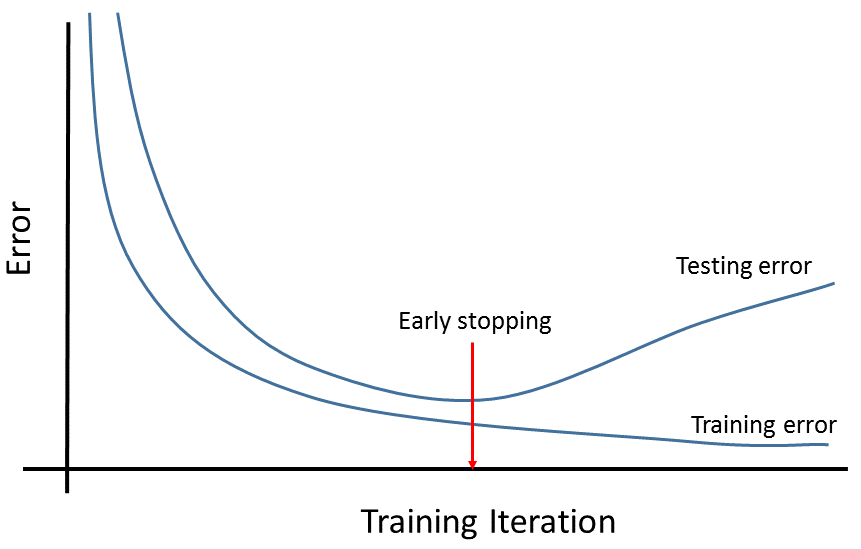
\includegraphics[width=0.85\linewidth]{images/training_testing_error_v2}
	\caption{Ideal training and testing error curves.}
	\label{fig:training_testing_error}
\end{figure}

\subsection{Convolution Neural Networks}

Convolution neural networks (CNNs) use convolutional filters instead of weights. They have been used in image processing. 

One of the first CNN architectures was LeNet-5 \cite{Lecun1998}. LeNet-5 classified 32x32 images of handwritten digits using two convolution-average pooling layers followed by two dense layers and an output. 

AlexNet \cite{Krizhevsky2012} was the first exploration into wider and deeper CNNs. 

Much more work has been done furthering CNNs. VGG \cite{Simonyan2014} showed that smaller filter sizes are good. 

\section{Autoencoders} \label{Autoencoders}
% \cite{CHARTE2018} is a practical guide to autoencoders. Great resource.

Autoencoders were introduced by Hinton \cite{Hinton2006}. They can be used as a method to pre-train networks or as feature extractors \cite{CHARTE2018}.

Other feature extraction methods exist. Principal component analysis (PCA) attempts to reduce the dimensionality of a dataset into linearly uncorrelated variables \cite{Jolliffe2002}. Using a few of these principle components, the data may be represented in a reduced space that contains most of the information present in the original data. Another linear feature extraction method is called linear discriminant analysis (LDA). LDA is a supervised feature extraction method that finds linear combinations of features that can be used to separate classes. Non-linear feature extraction methods, such as kernel PCA, also exist. Kernel PCA applies a non-linear transform to the input space and applies PCA to the data in this transformed space. For kernel PCA to perform well, the correct kernel must be chosen for a given problem, which is a non-trivial task.

Denoising was suggested as a method of extracting useful features from an autoencoder \cite{Vincent2008, Vincent2010}.

\cite{Masci2011} demonstrated that stacking convolution layers made a good autoencoder.

% While autoencoders were touched on in the uranium enrichment work, they have not been explored thoroughly. There is some evidence that the autoencoder was overtrained to the A special case of denoising autoencoders will be explored for the ANSI dataset. 

An autoencoder is an ANN whose goal is to learn a representation of the input. This is accomplished by simultaneously training an encoding ANN and a decoding ANN. An example of this can be seen in Figure \ref{fig:Autoencoder_structure}. As seen in this figure, the encoding ANN reduces an $n-$dimension input signal, $X$, to a $m-$dimension signal, $z$, where $m < n$. The decoding ANN takes the encoded signal, $z$, and outputs a reproduction of the input signal, $X'$.

Without an autoencoder, a single ANN has to learn multiple tasks to identify isotopes. An ANN would have to simultaneously identify the detector calibration, background signal, and possible source signal. By training an autoencoder to reconstruct a background-subtracted and correctly calibrated spectrum, the task of isotope identification is simplified for the ANN. This may result in more accurate identifications. To test this, for each dataset a single autoencoder and three ANNs will be trained. The first will be trained without an autoencoder. The second will be trained using the encoder as input. The third will be trained using the full autoencoder as input. A random hyperparameter search will be used to find an appropriately structured autoencoder. The testing and validation error for these ANNs will be compared for each respective dataset.

% is local spatial structure too much jargon? 
In addition to using fully connected autoencoders, a 1-D convolutional autoencoder will also be explored. A DNN does not assume the input has local spatial structure, while a CNN does. Because gamma-ray spectra have local spatial structure in the form of photopeaks and Compton continua, it may be better to use a CNN over a DNN \cite{CHARTE2018}. To test this, the experiment described above will be repeated using a 1-D convolutional autoencoder.

% Or I might just use the 1D convolutional autoencoder because it makes more sense

\begin{figure}[H]
\centering
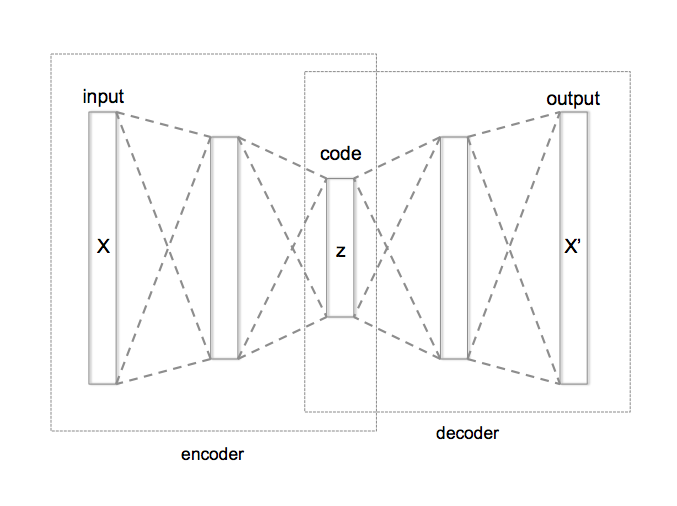
\includegraphics[width=0.8\linewidth]{images/Autoencoder_structure}
\caption{An example of an autoencoder \cite{wiki:AutoencoderStructure}.}
\label{fig:Autoencoder_structure}
\end{figure}


% Fully connected ANNs do not assume there is local spatial structure in a signal, so the fully connected ANN would need to learn that there is local structure. Convolutional ANNs assume there is local structure, and the extent of this structure can be changed by changing the length of the convolutional ANNs filters.

% Once the autoencoder is trained, the hidden layer and output layer (representing the reconstructed spectrum) will be used to train a separate ANN for isotope identification and quantification. The performance of these ANNs will be compared.



\subsection{Hyperparameters}

In addition to the weights connecting neurons, ANNs can have additional hyperparameters. Hyperparameters determine both the networks structure (number of layers, number of nodes in each layer, activation function for each layer) and how the model learns (learning rate, momentum, loss function). In the following section, various hyperparameters and their effects on ANN learning are discussed.

\subsubsection{Learning Rate}

The learning rate is a tunable parameter that affects the magnitude of each weight update. If $\eta$ is too small, the network will learn slowly and training will be inefficient. If $\eta$ is too large, the network will fail to learn, either by converging to a non-extremum or by diverging. An example of a small and large learning rate are shown in Figure \ref{fig:Learning_rate_comparison} 

\begin{figure}[H]
	\centering
	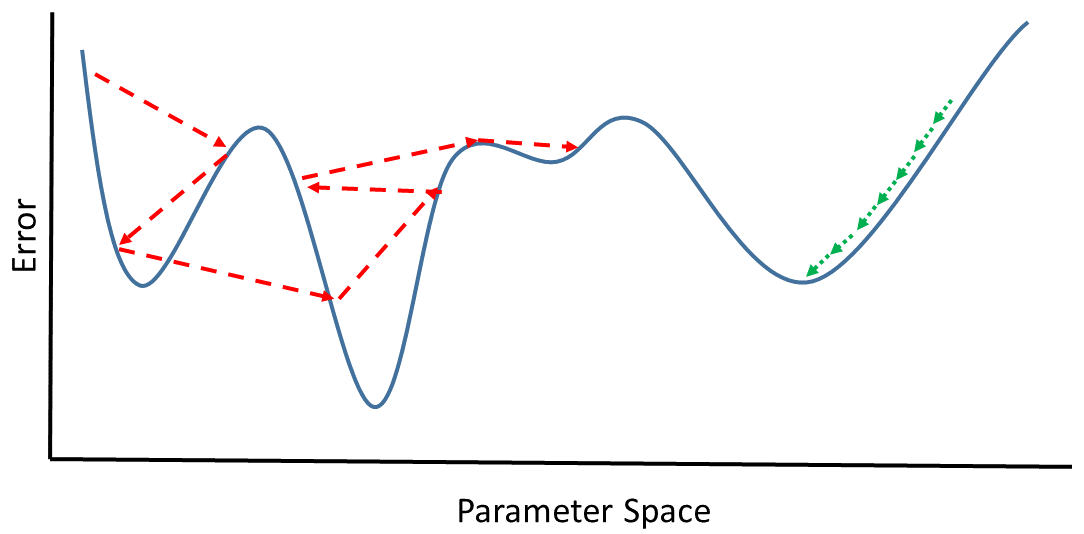
\includegraphics[width=0.8\linewidth]{images/Learning_rate_comparison_v2}
	\caption{Example training paths for a large learning rate, red, and a small learning rate, green.}
	\label{fig:Learning_rate_comparison}
\end{figure}


There are many methods to modify $\eta$ to encourage more efficient learning. One method to increase the speed of learning is to start with a large $\eta$ and decrease $\eta$ as a function of iteration number. Ideally, this method would lead to quick initial learning when far from an optima and slower learning near an optima to more finely explore it. The difficulty with this method is the requirement for a function that slows the learning rate efficiently for a given problem.

\subsubsection{Learning Momentum}

Another method to speed up learning is to add a momentum hyperparameter, $\mu$, to the weight update algorithm \cite{Yu1997}, 
%
\begin{equation} \label{eq:update_momentum}
\Delta w_{ij}(n) = - \eta \frac{dE_{MSE}}{dw_j} +\mu \Delta w_{ij}(n-1).
\end{equation}
%
Similar to the goal of slowing learning over time described above, the momentum term attempts to slow learning near optima. The momentum will be large when the weights are updated at large steps, far from an optima, but will decrease near an optima, allowing slower learning near an optimum.
 
\subsubsection{Training Algorithms}

There are many ANN training algorithms that employ clever learning rate schedules and momentum functions. These algorithms include but are not limited to: Nesterov's accelerated gradient \cite{nesterov1983}, simulated annealing \cite{Kirkpatrick1983}, ADADELTA \cite{ADADELTA}, and ADAM \cite{Kingma2015}. 

The ADAM optimizer was chosen as the training algorithm for the work presented in this thesis due to its incorporation of parts of other successful optimization algorithms and its reported superior performance over these algorithms. Another benefit of the ADAM optimizer is introduction of only one hyperparameter, the learning rate. 

The ADAM optimizer update rule is described below. For the following, $g_t$ is the gradient of the error function with respect to the network parameters at iteration $t$, 
\begin{equation} \label{eq:adam1}
m_t = \beta_1 m_{t-1} + (1 - \beta_1) g_t,
\end{equation}
is the estimate of the mean of the gradient at iteration $t$ and
\begin{equation} \label{eq:adam2}
v_t = \beta_2 v_{t-1} + (1 - \beta_2) g_t^2
\end{equation}
is the estimate of the variance of the gradient at iteration $t$. For the following, the variables $\beta_1$ and $\beta_2$ are parameters called decay rates, $\epsilon$ is another parameter, and $\theta_t$ represents the network parameters at iteration $t$. As described by Kingma and Lei Ba, The default values for $\beta_1$, $\beta_2$, and $\epsilon$ are 0.9, 0.999, and $10^{-8}$ respectively \cite{Kingma2015}. These values were seen to work well for a variety of problems. While these hyperparameters can also be tuned, it has been shown that the default values work well for a variety of network architectures and datasets \cite{Kingma2015}. The bias-corrected first moment estimate is given by
\begin{equation} \label{eq:adam3}
\hat{m}_t = \dfrac{m_t}{1 - \beta^t_1}
\end{equation}
and the bias-corrected second moment estimate is given by 
\begin{equation} \label{eq:adam4}
\hat{v}_t = \dfrac{v_t}{1 - \beta^t_2}.
\end{equation}
Finally, the weight update equation is computed as
\begin{equation} \label{eq:adam5}
\theta_{t+1} = \theta_{t} - \dfrac{\eta}{\sqrt{\hat{v}_t} + \epsilon} \hat{m}_t.
\end{equation}


%Due to the number of free parameters in a ANN (each hidden layer weight is a free parameter), these models have a tendency to overfit data. The three methods used to prevent overfitting in this thesis are $L_2$ regularization, neuron dropout, and data augmentation. These techniques greatly improve the performance of the presented ANN. 

% Is this neccesary? Just mentioning it is enough I think.

%Another method is to randomly perturbing the weights during training using a simulated annealing technique \cite{Kirkpatrick1983}. Simulated annealing mimics how crystal lattices bond together in cooling metal to achieve a low energy state. As metal cools, its crystal lattice will orient itself to lower its total bond energy, but occasionally due to statistical heating sections will jump to a higher energy level. This encourages a global low energy state, as many local low energy state regions are discouraged. This process can be mimicked in a learning algorithm by randomly perturbing the weights during learning. As learning continues the network 'cools' and the frequency of weight perturbation decreases. It can be shown that given a long enough annealing schedule, the global optimum solution for a problem is guaranteed to be found \cite{Granville1994}.

\subsubsection{Cost Function}

The choice of cost function to train against depends on the targets the network is attempting to learn. One of the simplest error functions is the binary accuracy for classification, 
%
\begin{equation} \label{eq:Binary_accuracy}
E_{Binary} = {\frac{1} N} \sum_{n=1}^N [\hat{y}_n \neq y_n ],
\end{equation}
%
where N is the total number of output neurons, $y_n$ is the ground truth of the n$^{th}$ output, and $\hat{y}_n$ is the ANN output of the n$^{th}$ output neuron. While this is a simple function, it penalizes the model for being close to the answer. Because there is no incremental indication that a model is improving, this error function is not typically used for gradient descent algorithms.

A simple differentiable cost function is the mean squared error (MSE) function shown in Equation \ref{eq:MSE_error}. This function is differentiable, so gradient descent algorithms can be applied to it. The MSE function is appropriate when targets are any real number, as in a regression problem. 
%
\begin{equation} \label{eq:MSE_error}
E_{Binary} = {\frac{1} N} \sum_{n=1}^N (\hat{y}_n - y_n)^2,
\end{equation}
%
For classification problems, the average cross entropy, shown in Equation \ref{eq:CrossEntropy} can be used. Cross entropy measures how different the probability distributions $y_n$ and $\hat{y}_n$ are from each other. Because the cross entropy treats $y_n$ and $\hat{y}_n$ as probability distributions, they are required to exist in the range [0,1].
%
\begin{equation} \label{eq:CrossEntropy}
E = -{\frac{1} N} \sum_{n=1}^N y_n \log(\hat{y}_n) +  (1-y_n) \log(1-\hat{y}_n), 
\end{equation}
%

Because the softmax function can be used for classification, it is traditionally used as the output function for the model when using the cross entropy cost function. The softmax function is used in binary classification problems to calculate posterior class probabilities \cite{Bridle1990}.

\begin{equation} \label{eq:softmax}
softmax(z_j) = \frac{\exp(z_j)} {\sum_{k=1}^{K} \exp(z_k)}.
\end{equation}


%% This part is kinda total butts
%It is important to note that for a single layer neural network with the MSE cost function, the one minimum in $MSE(W)$ is the global minimum. When the number of layers increases beyond one there may be many more local minima in the cost function. Care must be taken when training a neural network to either find the global minimum in the cost function with respect to the weights or to find a minimum that reduces the error below a desired value. Care must also be taken to avoid stuck training, or having the optimization algorithm find a local minimum and not move from it. A proper optimization technique must account for these pitfalls. 

\subsubsection{Weight Regularization}

Weight regularization is a hyperparameter that penalizes the ANN when the magnitude of the weights increases. Because the magnitude of the weights is tied to the complexity of the model, adding weight regularization attempts to limit complexity and the probability of overfitting.

A common method of incorporating weight regularization is by adding an $L_n$ regularization term to the error function, as seen in Equation \ref{eq:L2_Reg}. Common values for $n$ are 1 and 2. Adding weight regularization allows the magnitude of the weights to increase only when there is a comparable reduction in the unmodified error function.
%
\begin{equation} \label{eq:L2_Reg}
\tilde{E} = E + \sum_i \lambda w_i^n.
\end{equation}
%
In Equation \ref{eq:L2_Reg}, $w_i$ is the weight between each neuron in the ANN and $\lambda$ is the regularization strength hyperparameter. A larger $\lambda$ will force the ANN to prefer smaller weights connecting the neurons. If the parameter $\lambda$ is too small, the unbounded model complexity may fit only the training data. If the parameter $\lambda$ is too large, the ANN will only minimize the $L_n$ error, failing to learn.

\subsubsection{Neuron Dropout}

Another method to reduce model complexity is neuron dropout. Neuron dropout is the process of temporarily removing a neuron from the ANN architecture \cite{Srivastava2014}. By randomly removing neurons from an ANN during training, heavy local codependency between neurons that could lead to the ANN becoming stuck in a local minimum in the error function, and thus overtraining, is discouraged. The frequency with which neurons are removed is called the neuron dropout rate, which is a hyperparameter.

Almost always, taking the average output of more than one separately trained ANN improves the performance of the ANN \cite{Srivastava2014}. By applying dropout at each neuron with the same probability throughout training, the ANN's architecture changes every iteration. The makes neuron dropout a cost efficient way to effectively average many different ANN architectures, improving performance.

\subsubsection{Data Augmentation}

Data augmentation changes the data during training using physically realistic transformations. For example, a training dataset of images can be rotated, flipped, blurred, or color augmented during training. An example of horizontal flip and a blur augmentation are seen in Figure \ref{fig:cat}. This cheaply expands the training dataset and discourages overtraining, as the ANN never observes the exact same image. Both the augmentation method and strength of said method are hyperparameters. 

\begin{figure}[H]
	\centering
	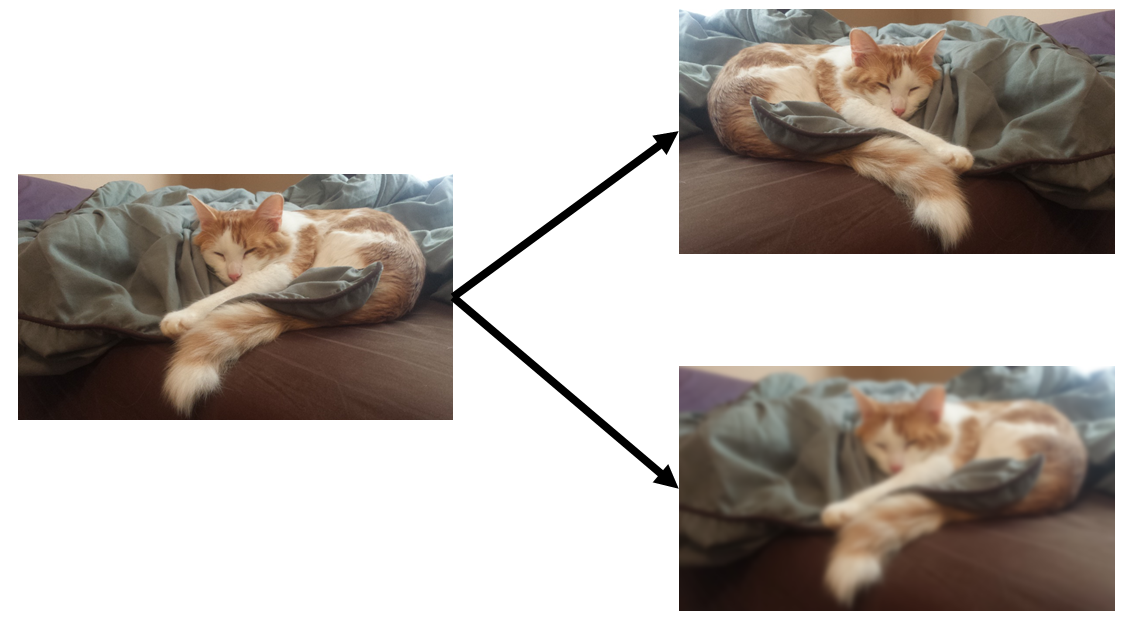
\includegraphics[width=0.9\linewidth]{images/cat}
	\caption{Two examples of data augmentation using an image of a cat. The image to the left is the original. The top right image is augmented using a horizontal flip. The bottom right image is augmented using blur.}
	\label{fig:cat}
\end{figure}

\subsection{Hyperparameter Optimization}

In general, ANNs have many hyperparameters that require optimization. Optimizing these hyperparameters will lead to more efficient training and more accurate performance when training is concluded. There are several different methods to perform hyperparameter optimization for an ANN. These methods may include manual optimization, exhaustive grid search, and random parameter search.

Manually optimizing parameters is necessary when developing a novel algorithm. This involves changing hyperparameters and observing how the ANN trains and the final error on a validation dataset. Ideally, the ANN should train quickly and have a low error on a validation dataset. For many parameters `rule of thumb' values exist that can be used to find parameters that work to some degree. Due to the large hyperparameter space, a manual search is cost prohibitive if further optimization is desired.

Once a range of parameters is determined through a manual search, multiple methods are available to explore the parameter space for an optimal solution. One method is an exhaustive grid search. In a grid search the parameter space is divided into a uniform grid and the joint performance of all parameters is tested. The grid search method is ineffective for two reasons. First, neural networks may have a large number of hyperparameters that need to be explored, and the computational requirement to explore the hyperparameter space increases exponentially with increasing hyperparamters. Second, in practice only a few hyperparameters dominate performance, but the dominating hyperparameters are different for different applications. A grid search may under represent the importance of key hyperparamters, as seen in Figure \ref{fig:Bergstra12a_hyperparameter_grid_vs_random}.  While this method works, it has been shown that a random search in the hyperparameter target domain finds better hyperparameters quicker than testing equally distributed points in the chosen range \cite{Bergstra2012}. It can also be shown that given 60 random samples over some space with a finite minimum, the minimum of those 60 random samples is within 5\% of the true minimum with 95\% probability \cite{Zheng2015}. This means that given a range of hyperparameters, the best performing hyperparameter combination out of 60 randomly sampled points is very likely to be close to optimal. 

\begin{figure}[H]
	\centering
	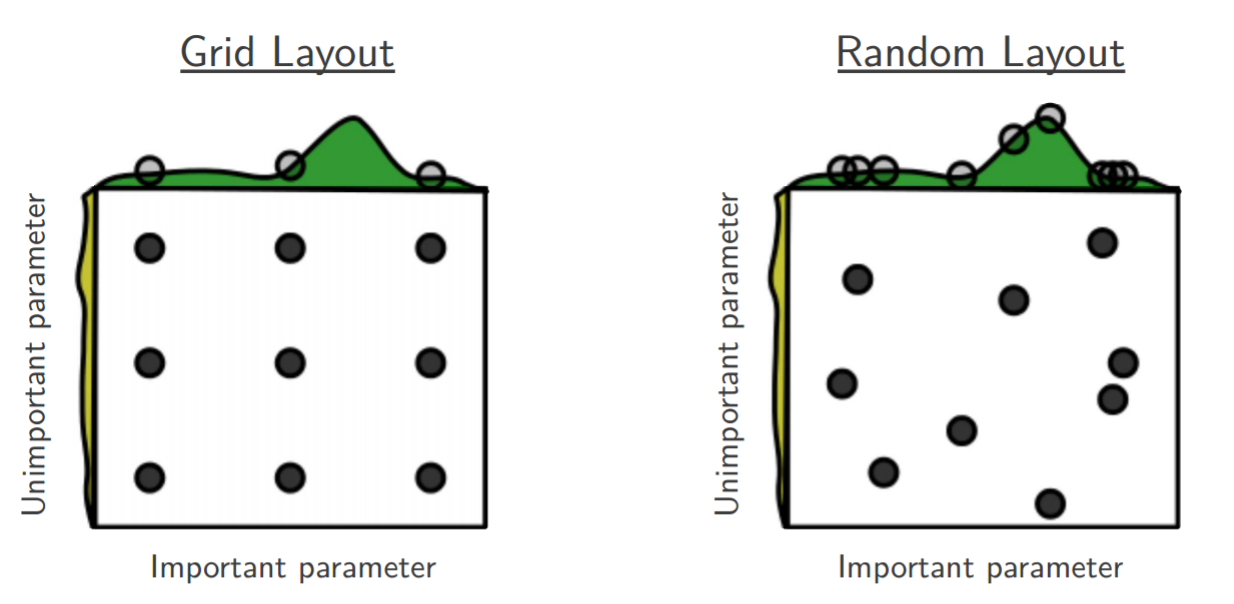
\includegraphics[width=0.99\linewidth]{images/Bergstra12a_hyperparameter_grid_vs_random}
	\caption{A comparison between a grid search and a random search for hyperparameter optimization when performance is strongly tied to one hyperparameter. The green function represents the effect of an important hyperparameter on a cost function while the yellow function represents the effect for an unimportant hyperparameter. Figure reproduced from [42].}
	\label{fig:Bergstra12a_hyperparameter_grid_vs_random}
\end{figure}


The ability for an ANN to solve a problem depends on the network structure, teaching method, and the training set to be learned. In the following section, a method for generating a training set for isotope identification and quantification is described.

To analyze the performance of a random search, a random hyperparameter efficiency curve, example shown in Figure \ref{fig:Bergstra_random_efficiency_curve_DNN} can be used. In the figure, 256 hyperparameter searches are run. These trials are split into experiments with sizes of increasing powers of two. The best performing trial from each experiment is determined and shown using a box plot.


\begin{figure}[H]
	\centering
	\includegraphics[width=0.9\linewidth]{model_choice_hyperparameter_search_images/Bergstra12_random_efficiency_curve}
	\caption{Example Random efficiency curves for a neural network \cite{Bergstra2012}.}
	\label{fig:Bergstra_random_efficiency_curve_DNN}
\end{figure}



\section{Summary}

In this chapter, the structure of multi-layer ANNs, methods to train and optimize them, and a method to create a training set for isotope identification and quantification have been described. In the following section an ANN will be presented using these concepts and its performance on a number of real and simulated spectra will be discussed. 













\chapter{Machine Learning Models Explored}

This section describes the structure of each machine learning models used for various gamma-ray spectroscopy tasks. The simplest model explored is the DNN. Because of the high dimension of the input data, feature extraction methods will be implemented and compared. These methods include PCA, a DAE, and a CAE. 

The other general architecture that will be explored is a 1D CNN. 


\section{Dataset Used for the Hyperparameter Search}

In order to find optimal hyperparameters, a dataset is required. Because searching for optimal hyperparameters for each different dataset is infeasible due to computational cost, a simplified gamma-ray spectroscopy dataset will be used to optimize network hyperparameters. The dataset is comprised of unshielded gamma-ray spectra of ANSI isotopes simulated using GADRAS. A total of 125 spectra are simulated for each isotope. Each spectrum has parameters randomly selected from Table \ref{table:hyperparameter_dataset_parameters}. From this dataset, 25\% of samples are randomly chosen as the test dataset. Early stopping with a patience of 20 epochs is used to train each network. The maximum number of epochs was set to 200.

\begin{table}[H]
\centering
\caption{Range of parameters used for the hyperparameter search dataset.}
\label{table:hyperparameter_dataset_parameters}
\begin{tabular}{l|c|c|}
\cline{2-3}
 & \multicolumn{1}{r|}{Minimum} & \multicolumn{1}{l|}{Maximum} \\ \hline
\multicolumn{1}{|l|}{Integration Time {[}s{]}} & 60 & 3600 \\ \hline
\multicolumn{1}{|l|}{Linear Calibration Offset} & 0.8 & 1.2 \\ \hline
\multicolumn{1}{|l|}{Signal to Background Ratio} & 0.5 & 3.0 \\ \hline
\end{tabular}
\end{table}


\section{Hyperparameter Search Results}

The results of the hyperparameter searches are shown using a few random efficiency curves. These curves allow for reproducibility. These also allow for researchers who want to fit models to this dataset to have a performance benchmark. If you wanted to compare random hyperparameter search to more intelligent methods, you could compare using this.

\subsection{Dense Architecture}

Architecture and training hyperparamters are shown in Table \ref{table:hyperparameter_dataset_parameters}. Note, the number of nodes in each layers was made to decrease for each subsequent layer.

\begin{table}[H]
\centering
\caption{Range of hyperparameter explored for the DNN.}
\label{table:hyperparameter_dataset_parameters}
\begin{tabular}{l|c|c|c|}
\cline{2-4}
 & \multicolumn{1}{r|}{Minimum} & \multicolumn{1}{l|}{Maximum} & Sampling Method \\ \hline
\multicolumn{1}{|l|}{Number of Layers} & 1 & 3 & Uniform \\ \hline
\multicolumn{1}{|l|}{Nodes in Layer} & 10 & 1000 & Logarithmic \\ \hline
\multicolumn{1}{|l|}{Initial Learning Rate} & 10$^{-4}$ & 10$^{-1}$ & Logarithmic \\ \hline
\multicolumn{1}{|l|}{L2 Regularization Strength} & 10$^{-2}$ & 10$^{1}$ & Logarithmic \\ \hline
\multicolumn{1}{|l|}{Batch Size} & 16 & 512 & Power of Two \\ \hline
\multicolumn{1}{|l|}{Activation Function} & \multicolumn{2}{c|}{tanh, sigmoid, relu} & Uniform \\ \hline
\end{tabular}
\end{table}



Random efficiency curves for different reprocessing methods for the DNN are shown in Figure \ref{fig:random_efficiency_curve_DNN_preprocessing}. This figure implies that the optimum prepossessing step is BLANK. It's interesting that BLANK does better than BLANK. 

In addition to hyperparameters associated with the DNN's architecture and training, hyperparameters explored include the autoencoder used. Autoencoders can generate a different encoding based on a given architecture. The mean squared reconstruction error may not be the best metric to measure how good this encoding is as a preprocessing step. To determine an optimum preprocessing architecture for the dense and convolutional autoencoder, the choice of preprocessing architectures was added as a hyperparameter. The choices belong to the set with the N best reconstruction errors, respective of dense and convolution architecture.

\subsubsection{Hyperparameter Search Results - Autoencoders}

Now that we know optimized autoencoder architectures for the DNN, we need to optimize training hyperparameters. 

% https://machinelearningmastery.com/activation-regularization-for-reducing-generalization-error-in-deep-learning-neural-networks/

% \cite{Ranzato2007} Fig 6 shows you can freeze the unsupervised feature extraction network and update the classifier if you have enough data.

Sparse denoising autoencoders are included in in this work as feature extraction and dimension reduction techniques. Both autoencoders employ regularization techniques to ensure useful representations are learned. Both models includes $l1$ activity regularization as a method to induce sparsity on the networks activations, which increases generalization \cite{Goodfellow-et-al-2016}. 

Show how well autoencoders worked at spectrum reconstruction and background subtraction. See if there's a large difference between doing background subtraction and 



\begin{figure}[H]
	\centering
	\includegraphics[width=0.8\linewidth]{model_choice_hyperparameter_search_images/Bergstra12_random_efficiency_curve}
	\caption{Random efficiency curves for the DAE. Sample curve from Bergstra 2012.}
	\label{fig:random_efficiency_curve_DAE}
\end{figure}


\begin{figure}[H]
	\centering
	\includegraphics[width=0.8\linewidth]{model_choice_hyperparameter_search_images/Bergstra12_random_efficiency_curve}
	\caption{Random efficiency curves for the CAE. Sample curve from Bergstra 2012.}
	\label{fig:random_efficiency_curve_CAE}
\end{figure}

\subsubsection{Hyperparameter Search Results - Dense architecture with preprocessing }

\begin{figure}[H]
	\centering
	\includegraphics[width=0.99\linewidth]{model_choice_hyperparameter_search_images/Bergstra12_random_efficiency_curve_DNN}
	\caption{Random efficiency curves for the DNN with different fixed preprocessing steps. Sample curve from Bergstra 2012.}
	\label{fig:random_efficiency_curve_DNN_preprocessing}
\end{figure}

Because we know the optimum network using the preprocessing as fixed, we know optimum architectures for the autoencoders. We can now find, given all the autoencoder choices, which preprocessing technique should be better overall for the DNN. To do this we re-run the hyperparameter search with preprocessing included as a hyperparameter. These architectures and training hyperparameters will be used as the final  DNN model.

\begin{figure}[H]
	\centering
	\includegraphics[width=0.8\linewidth]{model_choice_hyperparameter_search_images/Bergstra12_random_efficiency_curve}
	\caption{Random efficiency curves for the DNN with preprocessing steps as hyperparameters. Sample curve from Bergstra 2012.}
	\label{fig:random_efficiency_curve_DNN}
\end{figure}



\subsection{Convolution Architecture}

Just like the autoencoder, this can be done in one or two steps. One step: Train and optimize the entire network, convolution and dense layers. Two steps: Train and optimize the dense layer, using random initialization for non-trainable convolution filters. We'll probably go with the two-step.


\begin{figure}[H]
	\centering
	\includegraphics[width=0.8\linewidth]{model_choice_hyperparameter_search_images/Bergstra12_random_efficiency_curve}
	\caption{Random efficiency curves for the CNN, using non-trainable convolution filters. Sample curve from Bergstra 2012.}
	\label{fig:random_efficiency_curve_CAE}
\end{figure}




\begin{figure}[H]
	\centering
	\includegraphics[width=0.8\linewidth]{model_choice_hyperparameter_search_images/Bergstra12_random_efficiency_curve}
	\caption{Random efficiency curves for the CNN with final convolution archetecture. Sample curve from Bergstra 2012.}
	\label{fig:random_efficiency_curve_CAE}
\end{figure}








\section{Summary of Final Model Architectures}

Learning curves are [definition, explanation]. Learning curves are used to determine a few things. We will use them to do [the following].

First, They are used as a sanity check, to make sure we are sampling our input space with enough granularity. To know we are sampling well enough, we should be sampling in a region where the curves are flat for both algorithms.

Secondly, Learning curves give us insight into which algorithm works better on the hyperparameter optimization dataset and simple version of the problem. We're expecting the CNN to outperform the DNN due to theoretical benefits of convolution architectures for our problem. We can also compare this curve to the final learning curves for the final datasets.



% Show learning curve to determine how many samples to add
\begin{figure}[H]
	\centering
	\includegraphics[width=0.8\linewidth]{model_choice_hyperparameter_search_images/learning_curve_dummy}
	\caption{Learning curves from the best DNN and CNN. X-axis will change to number of (input space sampling granularity? input space sampling divisions?). Shown: learning curve example.}
	\label{fig:Node}
\end{figure}









% More or less Methods

\chapter{Urban Source Identification Results and Discussion}

% Compare how well we identify shielded/unshielded isotopes when training set has shielding, doesn't have shielding. 

% Compare how well we identify isotopes over different distances if training set has one vs many distances

% Compare how well we identify isotopes with different calibration sampling granularity 


\section{Problem Description and Training Dataset Overview}

This chapter applies machine learning algorithms to solve the problem of a identifying a radioactive source in an urban environment where a source may be present. This scenario is applicable when performing source interdiction searching cargo containers, vehicles at boarder crossings, or security at high profile events. Urban environments present unique challenges to gamma-ray spectroscopy. Background radiation can change over city blocks due to different concentrations of uranium and thorium in building materials. Sources may be purposely shielded by unknown amounts of material to obscure their gamma-ray signal.


\subsection{Training Dataset Overview}

The dataset is simulated using GADRAS-DRF (detector response function), a one-dimension particle transport code developed at Sandia National Laboratory. To create the dataset .

Spectra change due to changes in source-to-detector distance. These changes are due to changing scattering geometry, which can affect the peak-to-total ratio. These changes may have a large impact on identification performance. To incorporate these changes, templates simulated at different distances are included in the dataset. These distances start at 30cm, which is the distance at which a 1 uCi source will have an activity of about 400 cps on a 2 inch diameter detector. This is about twice the expected activity of background. 

Changes in calibration due to temperature shifts are also considered. Due to the relatively large magnitude in calibration shifts due to temperature shifts from -5 C to 40 C, it is expected incorporating these additions will also make the algorithm robust against calibration. If a As seen in \ref{fig:CASANOVAS2012588}, 




\section{Results from training all models}

When training final models, two main questions need to be addressed: how good is a given architecture at solving a problem on its training dataset and how good is a given dataset at generalizing to outside examples.

To determine how good a given architecture solves a problem, asymptotic convergence of the models performance needs to be measured. Because of the inherent stochastic nature of training machine learning algorithms (different random weight initialization, different mini-batches chosen during training, different data augmentation manifestations), each time a new network is trained the networks parameters and results will differ. This means a single trained instance of some model A may outperform a single trained instance of model B by chance, despite model B being an overall superior architecture. To more realistically compare how models perform on some dataset, a number of networks can be trained and their average performance compared. This is a method called bagging.

\subsection{Asymptotic Model Performance on Training Dataset}

For the best DNN and CNN architectures found in the hyperparameter search, using 'enough' data data samples as found in the hyperparameter search, 30 networks are trained. Their performance is observed in Figure \ref{fig:asymptotic_performance}.


%% Can also include performance using templates with extreme augmentation
\begin{figure}[H]
	\centering
	\includegraphics[width=0.8\linewidth]{model_choice_hyperparameter_search_images/asymptotic_performance_dummy}
	\caption{Asymptotic model performance for both the CNN and DNN on the training sets.}
	\label{fig:asymptotic_performance}
\end{figure}

Using N models as representative of asymptotic performance, justified in Figure \ref{fig:asymptotic_performance}, we can check out the confusion matrix associated with the test dataset to gain insight into how the algorithm is performing poorly and predict future shortcomings.


%% Can also include performance using templates with extreme augmentation
\begin{figure}[H]
	\centering
	\includegraphics[width=0.8\linewidth]{model_choice_hyperparameter_search_images/conf_matrix_example}
	\caption{Asymptotic model performance for both the CNN and DNN on the training sets.}
	\label{fig:asymptotic_performance}
\end{figure}

% Can also analyze how changing a threshold would affect precision/recall!

% \subsection{Results from training models using extreme data augmentation vs Data Augmentation grid sampling}

% Show learning curve between models 
% Instead of training examples on x-axis, plot against "number of divisions" (which also has a number of training examples included...)
% Note! You can start holding parameters constant to see what parameter the model is having difficulty explaining
% \begin{figure}[H]
%	\centering
%	\includegraphics[width=0.8\linewidth]{model_choice_hyperparameter_search_images/learning_curve_dummy}
%	\caption{Learning curve example.}
%	\label{fig:Node}
%\end{figure}

%% Plot of average F1-score vs epochs for all models. Datasets include different detector model (use this as validation set) and same detector model with certain augmentation parameters frozen (or just the training set).


%% Plot of average F1-score vs epochs for all models. Datasets include different detector model (us this as validation set) and same detector model with certain augmentation parameters frozen (or just the training set).

\subsection{Results on Spectra for ANSI compliance}

This section shows model asymptotic performance vs integration time for ANSI compliance. Using N models (justified previously as asymptotic). 


% List Represents table of 
\begin{itemize}
  \item $^{137}$Cs + depleted uranium (DU)
  \item $^{99m}$Tc + HEU
  \item $^{201}$Tl + HEU
  \item $^{67}$Ga + HEU
  \item $^{131}$I + WGPu
  \item Naturally occurring radioactive material (NORM) + HEU
  \item NORM + WGPu
\end{itemize}


\subsection{Results on Measured Spectra}

This section shows model asymptotic performance vs integration time for a few different settings (different voltages, shielding)

\subsubsection{Asymptotic Model Performance on Changing Voltage}

To see the generalization performance of the model to changing calibration, spectra with different voltages are recorded and their asymptotic performance compared.

Figures \ref{fig:model_asymptotic_performance_co60} and \ref{fig:model_asymptotic_performance_cs137} show performance for isotopes with comparatively simple spectra.

\begin{figure}[H]
	\centering
	\includegraphics[width=0.75\linewidth]{model_choice_hyperparameter_search_images/asymptotic_performance_time}
	\caption{Asymptotic model performance for both the CNN and DNN on voltage vs integration time for $^{60}$Co.}
	\label{fig:model_asymptotic_performance_co60}
\end{figure}

\begin{figure}[H]
	\centering
	\includegraphics[width=0.75\linewidth]{model_choice_hyperparameter_search_images/asymptotic_performance_time}
	\caption{Asymptotic model performance for both the CNN and DNN on voltage vs integration time for $^{137}$Cs.}
	\label{fig:model_asymptotic_performance_cs137}
\end{figure}

Figures \ref{fig:model_asymptotic_performance_eu152} and \ref{fig:model_asymptotic_performance_ba133} show performance for isotopes with comparatively complicated spectra.

\begin{figure}[H]
	\centering
	\includegraphics[width=0.75\linewidth]{model_choice_hyperparameter_search_images/asymptotic_performance_time}
	\caption{Asymptotic model performance for both the CNN and DNN on voltage vs integration time for $^{152}$Eu.}
	\label{fig:model_asymptotic_performance_eu152}
\end{figure}

\begin{figure}[H]
	\centering
	\includegraphics[width=0.75\linewidth]{model_choice_hyperparameter_search_images/asymptotic_performance_time}
	\caption{Asymptotic model performance for both the CNN and DNN on voltage vs integration time for $^{133}$Ba.}
	\label{fig:model_asymptotic_performance_ba133}
\end{figure}

\subsubsection{Asymptotic Model Performance on Changing Shielding}

\begin{figure}[H]
	\centering
	\includegraphics[width=0.75\linewidth]{model_choice_hyperparameter_search_images/asymptotic_performance_time}
	\caption{Asymptotic model performance for both the CNN and DNN on shielding vs integration time.}
	\label{fig:asymptotic_performance}
\end{figure}



\subsubsection{Spectra with a Single Isotope}

\subsubsection{Spectra with a Isotope Mixtures}

% Super crazy, check out effect of changing ID threshold on F1 score for these data. Or, using optimum threshold found before, check out 

The ANNs ability to identify mixtures of less than three isotopes will be addressed. Mixtures of $^{60}$Co, $^{137}$Cs, $^{152}$Eu, and $^{133}$Ba will be recorded. The mean ANN outputs and their variances will be reported.


\chapter{Uranium Enrichment Regression Results and Discussion}

\section{Problem Description and Training Dataset Overview}



\section{Results from Training all Models}

% Is it necessary to re-run the hyperparameter search, or are the 'simple' models good enough?

Asymptotic models are 


Again, measure asymptotic MSE convergence.


\chapter{Conclusions and Future Work}

\section{General Conclusions}


\section{Steps Towards Practical Application}

For this model to be applied in the real world, a few things need to be added. Overall, a larger more thorough validation dataset must be created to ensure certain isotope combinations do not present as adversarial. That is, a validation dataset must be used to ensure a threat isotope is not commonly identified as benign. Additional hyperparameter tests need to be preformed with more intelligent hyperparameter ranges. Additional network architectures and hyperparameters should be explored. These can include inception networks and batch normalization.

Generalization performance must also be more thoroughly measured and improved. To increase generalization, a wider range of scattering environments needs to be added to the spectral templates. More detector parameters need to be varied and their effect on performance must be measured. 



\section{Suggested Future Works}

% 80%+ Wish list 
Siamese networks for SNM identification. Step 1, train a siamese network on simulated SNM with realistic missile shielding. Step 2, take a random warhead and call it 'golden'. Compare all other warheads to this, using only the spectrum as input. Boom, got a zero-knowledge verification alg.
% Differentiate different enrichments of uranium? 
% Use it as a feature extractor!!!!!

Treating dataset expansion methods [calibration, signal-to-total ratio] as random data augmentation instead of sampling them discreetly. Compare asymptotic performance of this 'extreme data augmentation model' on template dataset to performance of 'dataset expansion models' at expansion levels sufficient for learning curve asymptote. 

Create training datasets composed of isotope mixtures. How to sample these mixtures? Exhaustive? Latin hypercube (this is my preference)? Uniform random? See how this works on single- and multi-isotope identification.

For the autoencoder, compare performance of a model using cross-entropy loss on data log-normalized and squished on [0,1] to a model using mean-squared-error loss on data log-normalized and data sqrt-normalized.

% True future work

 

Much of the gamma-ray spectrum has no information in it, there are no peaks in certain regions. You can apply different preprocessing techniques to shrink these sections (similar to what RSL has done). What is the effect of these re-calibrations on performance?

See how well kernel SVM, boosted trees, random forests work on features extracted by DAE, CAE, PCA. Do these methods perform better on the datasets I've provided compared to the neural networks I've demonstrated? Compare speed, accuracy on simulated and collected data.

Autoencoder that takes spectrum as input, output is peak positions. Use this as a feature extractor. 

Can you address background identification errors by adding a higher penalizing term to the cost of mislabeling background? How does this play with precision/recall/F1 score as you change the decision threshold?

A simulated training set also allows the same ANN creation process to be applied to different detector materials. This is because different gamma-ray detector materials, such as CZT or HPGe, create spectra with different features.

Construct a dataset to detect obscured sources. For example, make a dataset with different (theoretically identifiable) amounts of HEU hidden by industrial and medical sources. 

Can you create a dataset to perform online uranium enrichment using NaI for fuel fabrication plants? Need to incorporate centrifuge wall thickness, can possibly use time-series data to identify when things change? May need to worry more about calibration drift due to temperature or electronics drift.





%%%%%%%%%%%%%%%%%%%%%%%%%%%%%%%%%%%%%%%%%%%%%%%
%%%%%%%%%%%%%%%%%% APPENDIX %%%%%%%%%%%%%%%%%%%
%%%%%%%%%%%%%%%%%%%%%%%%%%%%%%%%%%%%%%%%%%%%%%%
\appendix
%\include{apx}

\backmatter
%%%%%%%%%%%%%%%%%%%%%%%%%%%%%%%%%%%%%%%%%%%%%%%
%%%%%%%%%%%%%%%% BIBLIOGRAPHY %%%%%%%%%%%%%%%%%
%%%%%%%%%%%%%%%%%%%%%%%%%%%%%%%%%%%%%%%%%%%%%%%
\bibliographystyle{IEEEtran} % Dunno what format they want this!!! -MK 9/19/16
\bibliography{refs.bib}



%%%%%%%%%%%%%%%%%%%%%%%%%%%%%%%%%%%%%%%%%%%%%%%
%%%%%%%%%%%%%%%%%%%%%%%%%%%%%%%%%%%%%%%%%%%%%%%

\end{document}
\endinput
